\section{\texttt{DifferentialPrivacyFilter}}
\label{Implementation:DifferentialPrivacy}

The concept of \textit{differential privacy} is introduced in~\sref{Theory:SDC:Guarantees:DifferentialPrivacy} and on~\sref{Theory:SDCMethods:LaplaceMechanism} a data release \textit{mechanism} that achieves this privacy guarantee is described: the Laplace mechanism. The drawback of differential privacy is that its definition relies on an interactive \textit{query-response} environment, which is definitely not the one we encounter in stream data mining. However, we can find in the literature some efforts to bring differential privacy to non-interactive settings, such as in~\citet{Leoni:NonInteractiveDiffPriv} and~\citet{Domingo:EnhancingDiffPrivMicroaggregation}. The \texttt{DifferentialPrivacyFilter} is devised to provide a differentialy private release method in such a setting, namely, in the context of MOA privacy filters.

\subsection{Design}
\label{Implementation:DifferentialPrivacy:Design}

Following the idea presented in~\citet{Domingo:EnhancingDiffPrivMicroaggregation}, we have built an SDC method which combines microaggregation with the Laplace mechanism. We recall now the definition of this mechanism:

\begin{definition}~(Laplace mechanisnm)\\
Given a dataset $X$ and a function $f : X \rightarrow \mathbb{R}^d$, with $w \in \mathbb{N}^+$, an $\varepsilon$-differential privacy mechanism $\mathcal{M}$ for releasing $f$ is to publish
\begin{equation*}
\mathcal{M}(X) = f(X) + L
\end{equation*}
where $L$ is a vector of $d$ random variables each drawn from a Laplace distribution $Lap(0,\frac{\Delta(f)}{\varepsilon})$.
\end{definition}

We must remember that the amount of noise introduced by the addition of $L$ to the application of $f$ depends on the \textit{sensitivity} of $f$, denoted by $\Delta (f)$, this is, the maximum variation in the result of $f$ when computed over two neighbour datasets, i.e., sets differing in at most one record. For a fixed $\varepsilon$, the higher the sensitivity of $f$, the more noise is added.

Let $I_r(X)$ be the function that returns the attribute values corresponding to the $r$-th record (instance) of a stream $X$, this is, the ``identity'' function that returns instances from a stream. It is clear that $I_r$, formally defined as 

\begin{equation}
	\begin{aligned}
	I : X \times \mathbb{N}^+ &\to \mathbb{R}^d\\
	(X,r) &\mapsto (x_{r1},x_{r2},...,x_{rd})
	\end{aligned}
\end{equation}

where $d \in \mathbb{N}^+$, $X$ a \textit{dataset} and $r \in \mathbb{N}$, is a good candidate to be fed into the Laplace mechanism to obtain an $\varepsilon$-differential private data release method.

The idea is now to compose $I_r$ with a microaggregation function $M$, this is, $I_r \circ M$ in order to reduce the sensitivity of the results, thus increasing the analytical utility of data released by the mechanism $\mathcal{M}(X) = (I_r \circ M)(X) + L$. If we are able to lower the sensitivity of the function captured by the Laplace mechanism, the information loss due to the noise added will also be lower.

As we will see in~\sref{Implementation:DifferentialPrivacy:Design:AllTogether}, the \texttt{DifferentialPrivacyFilter} implements the mechanism $\mathcal{M}$ described in the previous paragraph using the $I_r \circ M$ composition.

\subsubsection{Insensitive microaggregation}
\label{Implementation:DifferentialPrivacy:Design:InsensitiveMicroaggregation}

\citet{Domingo:EnhancingDiffPrivMicroaggregation} prove that, by using an \textit{insensitive microaggregation} function $M$, the global sensitivity of its composition with $I_r$ is $\Delta (I_r \circ M) \leq \Delta (I_r) / k$, being $k$ the minimum size of the clusters returned by $M$. The condition that such an \textit{insensitive} algorithm must fulfill is:

\begin{definition}~(Insensitive microaggregation~\citep{Domingo:EnhancingDiffPrivMicroaggregation})\\
Let $X$ be a dataset, $M$ a microaggregation algorithm, and let $\{C_1,...,C_n\}$ be the set of clusters that result from running $M$ on $X$. Let $X^*$ be a neighbour dataset of $X$, differing in a single record, and $\{C_1^*,...,C_n^*\}$ the clusters that result from running $M$ on $X^*$. We say that $M$ is insensitive to the input data if there is a bijection between the set of clusters $\{C_1,...,C_n\}$ and the set of clusters $\{C_1^*,...,C_n^*\}$ such that each corresponding pair of clusters differs at most in a single record.
\end{definition}

Microaggregation algorithms are, however, very sensitive to the input data, this is, concerning the previous definition, they mostly do not accomplish it, because a minimum change in a single record can cause the generation of completely different clusters. In order to correct this behaviour,~\citet{Domingo:EnhancingDiffPrivMicroaggregation} prove that the design of an insensitive microaggregation algorithm is possible by using a an \textit{order relation consistent} distance metric in the partition step.

\begin{definition}~(Order relation consistent distance~\citep{Domingo:EnhancingDiffPrivMicroaggregation})\\
A distance function $d : X \times X \rightarrow \mathbb{R}$ is said to be consistent with a order relation $\leq_{X}$ if $d(x,y) \leq d(x,z)$ whenever $x \leq_{X} y \leq_{X} z$.
\end{definition}

One way to achieve such a consistent distance function is to define a total order relation among the elements of a dataset $X$ as follows: given a \textit{reference point} $R \in X$, for a pair of elements $x,y \in X$, we say that $x \leq y$ if $d(R,x) \leq d(R,y)$, where $d$ is a function such that $d : Dom(X) \times Dom(X) \rightarrow \mathbb{R}$ (the Euclidean distance between records of $X$, for example). Furthermore, in order to increase the \textit{within-cluster} homogeneity (see~\sref{Theory:SDCMethods:Microaggregation}), this reference point $R$ should be located at the boundaries of $Dom(X)$.

\subsubsection{Sensitivity estimation}
\label{Implementation:DifferentialPrivacy:Design:Sensitivity}

In the previous section, we discussed how to achieve a reduction in the sensitivity of $I_r$ by composing it with an insensitive microaggregation function such that the following result holds: $\Delta (I_r \circ M) \leq \Delta (I_r) / k$.

The problem, however, remains in determining the actual sensitivity of $I_r$. By definition of sensitivity, the maximum change that occurs in $I_r$, as a result of a single record being different in the dataset $X$ on which $I_r$ is applied, can be estimated as the range of $Dom(X)$, when the attributes of $X$ are numerical. For example, if an attribute $a$ in a dataset represents the height of a person, and $Dom(a) = [a_{min},a_{max}]$, the difference in the result of $I_r$ that the presence or abscence of an individual in this dataset causes is bounded by the range $[a_{min},a_{max}]$. This is, however, a very naïve estimation, because it assumes that this attribute values in the dataset, are representative of the attribute values of the \textit{population}. Particularly, it means that the population outliers are represented in the dataset.

Despite being a very rough estimate, we will use it to scale the amount of noise added to the data that will eventually be released. More accurately, we will estimate the sensitivity of an attribute $j$ for the function $I_r$ over a dataset $X$ as

\begin{equation}
\Delta_j\big(I_r(X)\big) = 1.5 \times \Big(\max\big(Dom(X_j)) - \min\big(Dom(X_j))\Big)
\end{equation}

Notice that a scaling factor of 1.5 is applied, in order to make the estimation more reasonable. The idea of this estimation was also drawn from~\citet{Domingo:EnhancingDiffPrivMicroaggregation}.

\subsubsection{Putting it all together}
\label{Implementation:DifferentialPrivacy:Design:AllTogether}

Given a dataset $X$ with $m$ attributes, the \texttt{DifferentialPrivacyFilter} class implements the Laplace mechanism 

\begin{equation*}
\mathcal{M}(X) = (I_r \circ M)(X) + L
\end{equation*}

where $M$ is an insensitive $k$-microaggregation function and $L$ is a vector of random variables $l_j$, for $1 \leq j \leq m$, each drawn from a Laplace distribution $Lap_j(0,b_j)$, with $b_j$ being the scale parameter, estimated by

\begin{equation*}
b_j = \frac{\Delta_j\big(I_r(X)\big)}{\varepsilon}
\end{equation*}

A general and high level description of the complete mechanism, adapted to a streaming environment, is given in~\alref{al:laplace-mechanism}. Notice that a single instance is processed in the algorithm pseudo-code: the privacy filter executes the mechanism for each instance in the input data stream. All the involved classes and modules of the actual implementation can be seen in~\fref{fig:class-differential-privacy-filter}.

\begin{algorithm}[h]
\KwData{an instance $x$ from a stream, an insensitive microaggregation function $M$ and a Laplace noise adder $\mathcal{L}$}
\KwResult{an anonymized instance $x'$}
\Begin{
	$\mu \leftarrow M(x)$\;
	$x' \leftarrow \mathcal{L}(\mu)$\;
	\KwRet{$x'$}\;
}
\caption{Microaggregation-based Laplace Mechanism\label{al:laplace-mechanism}}
\end{algorithm}

\begin{figure}
	\centering
	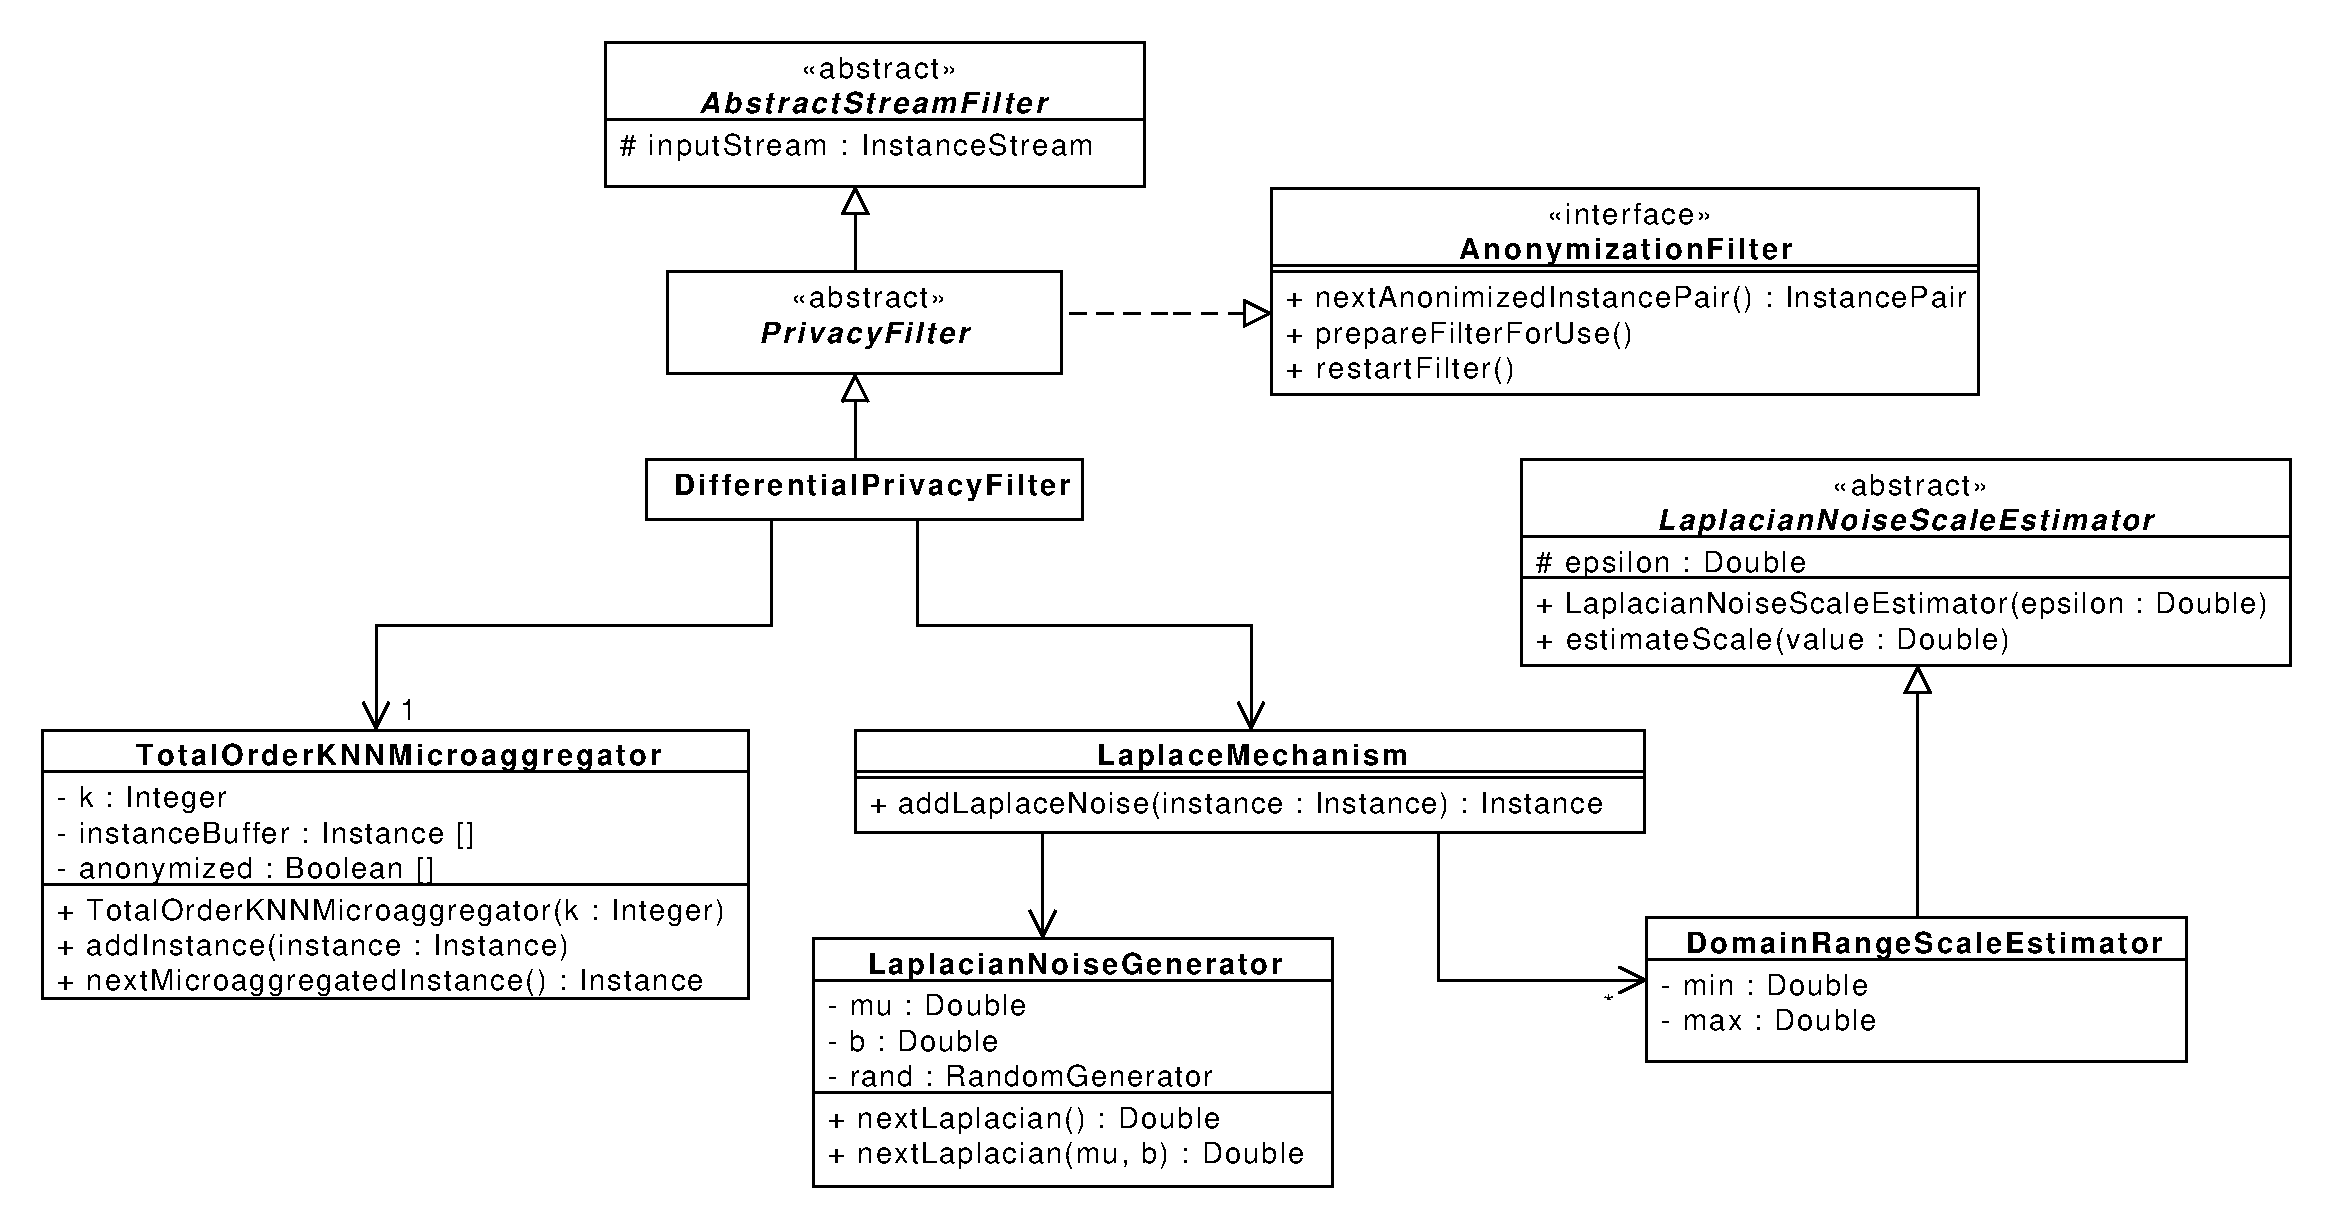
\includegraphics[width=1.0\linewidth]{figures/class_DifferentialPrivacyFilter.pdf}
	\caption[\texttt{DifferentialPrivacyFilter} class environment.]{\texttt{DifferentialPrivacyFilter} and the related classes and types it uses. Notice that the \texttt{LaplaceMechanism} uses many noise scale estimators, one for each attribute in the stream.}
	\label{fig:class-differential-privacy-filter}
\end{figure}

The adaptation of the insensitive microaggregation algorithm to a stream processing environment follows the same scheme presented for the \texttt{MicroAggregationFilter} (see~\sref{Implementation:Microaggregation:Design}), the only difference being the use of a \textit{reference} point in order to achieve a total ordering relation between the instances of the stream and, thus, fulfilling the insensitivity condition. The reference ``point'', denoted by $\mathcal{R}$, is incrementally\footnote{Remember that, in a stream processing environment, and more precisely, in the context of a \textit{buffered filter} (see~\sref{Implementation:BufferedFilter}), only a portion of the complete dataset (the stream) is visible to the algorithm at a given moment.} built as \textit{new} instances are processed by the filter, this is, it is updated independently of the clustering step, when a new instance is added to the buffer. The necessary modifications are presented in \alref{al:insensitive microaggregation}.

\begin{algorithm}[h]
\KwData{$W', A$ buffers and $\mathcal{R}$, the current reference point}
\KwResult{a \textit{cluster} $\mathcal{C}$ of $k$ instances}
\Begin{
	$\mathcal{C} \leftarrow \emptyset$\;
	$Q \leftarrow$ PriorityQueue$\langle$DistanceInstancePair$\rangle$()\;
	\For{$ x \in W', x \notin A $}{
		$d \leftarrow \mathrm{dist}(x,\mathcal{R})$\;
		$p \leftarrow$ DistanceInstancePair($d$, $x$)\;
		\eIf{$\vert Q \vert < k$}{
			$Q \leftarrow Q \cup p$\;
		}{
			\If{$p < Q$.peek().distance()}{
				$Q.poll()$\;
				$Q \leftarrow Q \cup p$\;
			}
		}
	}
	\For{$q \in Q$}{
		$\mathcal{C} \leftarrow \mathcal{C} \cup q.instance()$\;
	}
	\KwRet $\mathcal{C}$\;
}
\caption{KNN-based Insensitive Clustering\label{al:insensitive microaggregation}}
\end{algorithm}

The Laplace-distributed noise addition step of the mechanism is performed by a noise adder (called $\mathcal{L}$ in~\alref{al:laplace-mechanism}) that works in a very similar fashion to the \texttt{NoiseAdditionFilter}, with the addition of the scale parameter estimation, already discussed before. The complete description of the procedure is given in~\alref{al:laplace-noise-adder} and, finally, the generation of a random variable $\Lambda$ following a Laplace distribution is shown in the equation below:

\begin{equation}
\Lambda \sim Lap(\mu,b) \iff \Lambda = \mu - b~\mathrm{sgn}(U)~\ln(1-2\vert U \vert)
\end{equation}

where $U$ is another random variable drawn from a uniform distribution constrained to the $(-0.5,0.5]$ interval.

\begin{algorithm}
\KwData{an instance $x$ and a vector $B$ of scale estimators}
\KwResult{an anonymized instance $x'$}
\Begin{
	\For{$i \in \mathrm{attributes}(x)$}{
		$b \leftarrow B_i.estimate(x_i)$\;
		$x_i' \leftarrow x_i + \mathrm{Random}.laplace(0,b)$\;
	}
	\KwRet{$x'$}\;
}
\caption{Laplace Noise Adder\label{al:laplace-noise-adder}}
\end{algorithm}